\subsection{Tiempo de ejecución}

En el análisis de los resultados experimentales, se muestra el tiempo 
promedio de cada algoritmo en función del tamaño de la 
grilla ($n \times m$ celdas), con ambos ejes en escala 
logarítmica. El tiempo en fuerza bruta crece de forma exponencial: 
en grillas libres pasa de aproximadamente $12$ ms en $8 \times 16$ 
a aproximadamente $7$ s en $16 \times 16$, un factor de aproximadamente $600$, 
que es del orden de la cantidad de caminos posibles (aproximadamente $910$). 
Según como sea el terreno, el tiempo en $16 \times 16$ varía entre 
$2$ y $8$ segundos aproximadamente. Por esta razón solo se 
ejecutó con $N+M \le 32$.

\vspace{0.4cm}

Por otro lado, la programación dinámica crece con pendiente de aproximadamente $1$ 
en escala log-log, consistente con $\mathcal{O}(n \cdot m \cdot v)$, 
y resuelve $1024 \times 2048$ en aproximadamente $0{,}6$ s. 
Greedy crece mucho más lento, resuelve $1024 \times 2048$ 
en aproximadamente $0{,}3$ ms, acorde a $\mathcal{O}(n+m)$, y es 
unas $2000$ veces más rápido que DP en ese tamaño. 
En grillas muy pequeñas DP y greedy son muy similares 
(con tiempos de aproximadamente $10^{-2}$ ms) porque domina el costo fijo de 
la medición.

\begin{figure}[H]
    \centering
    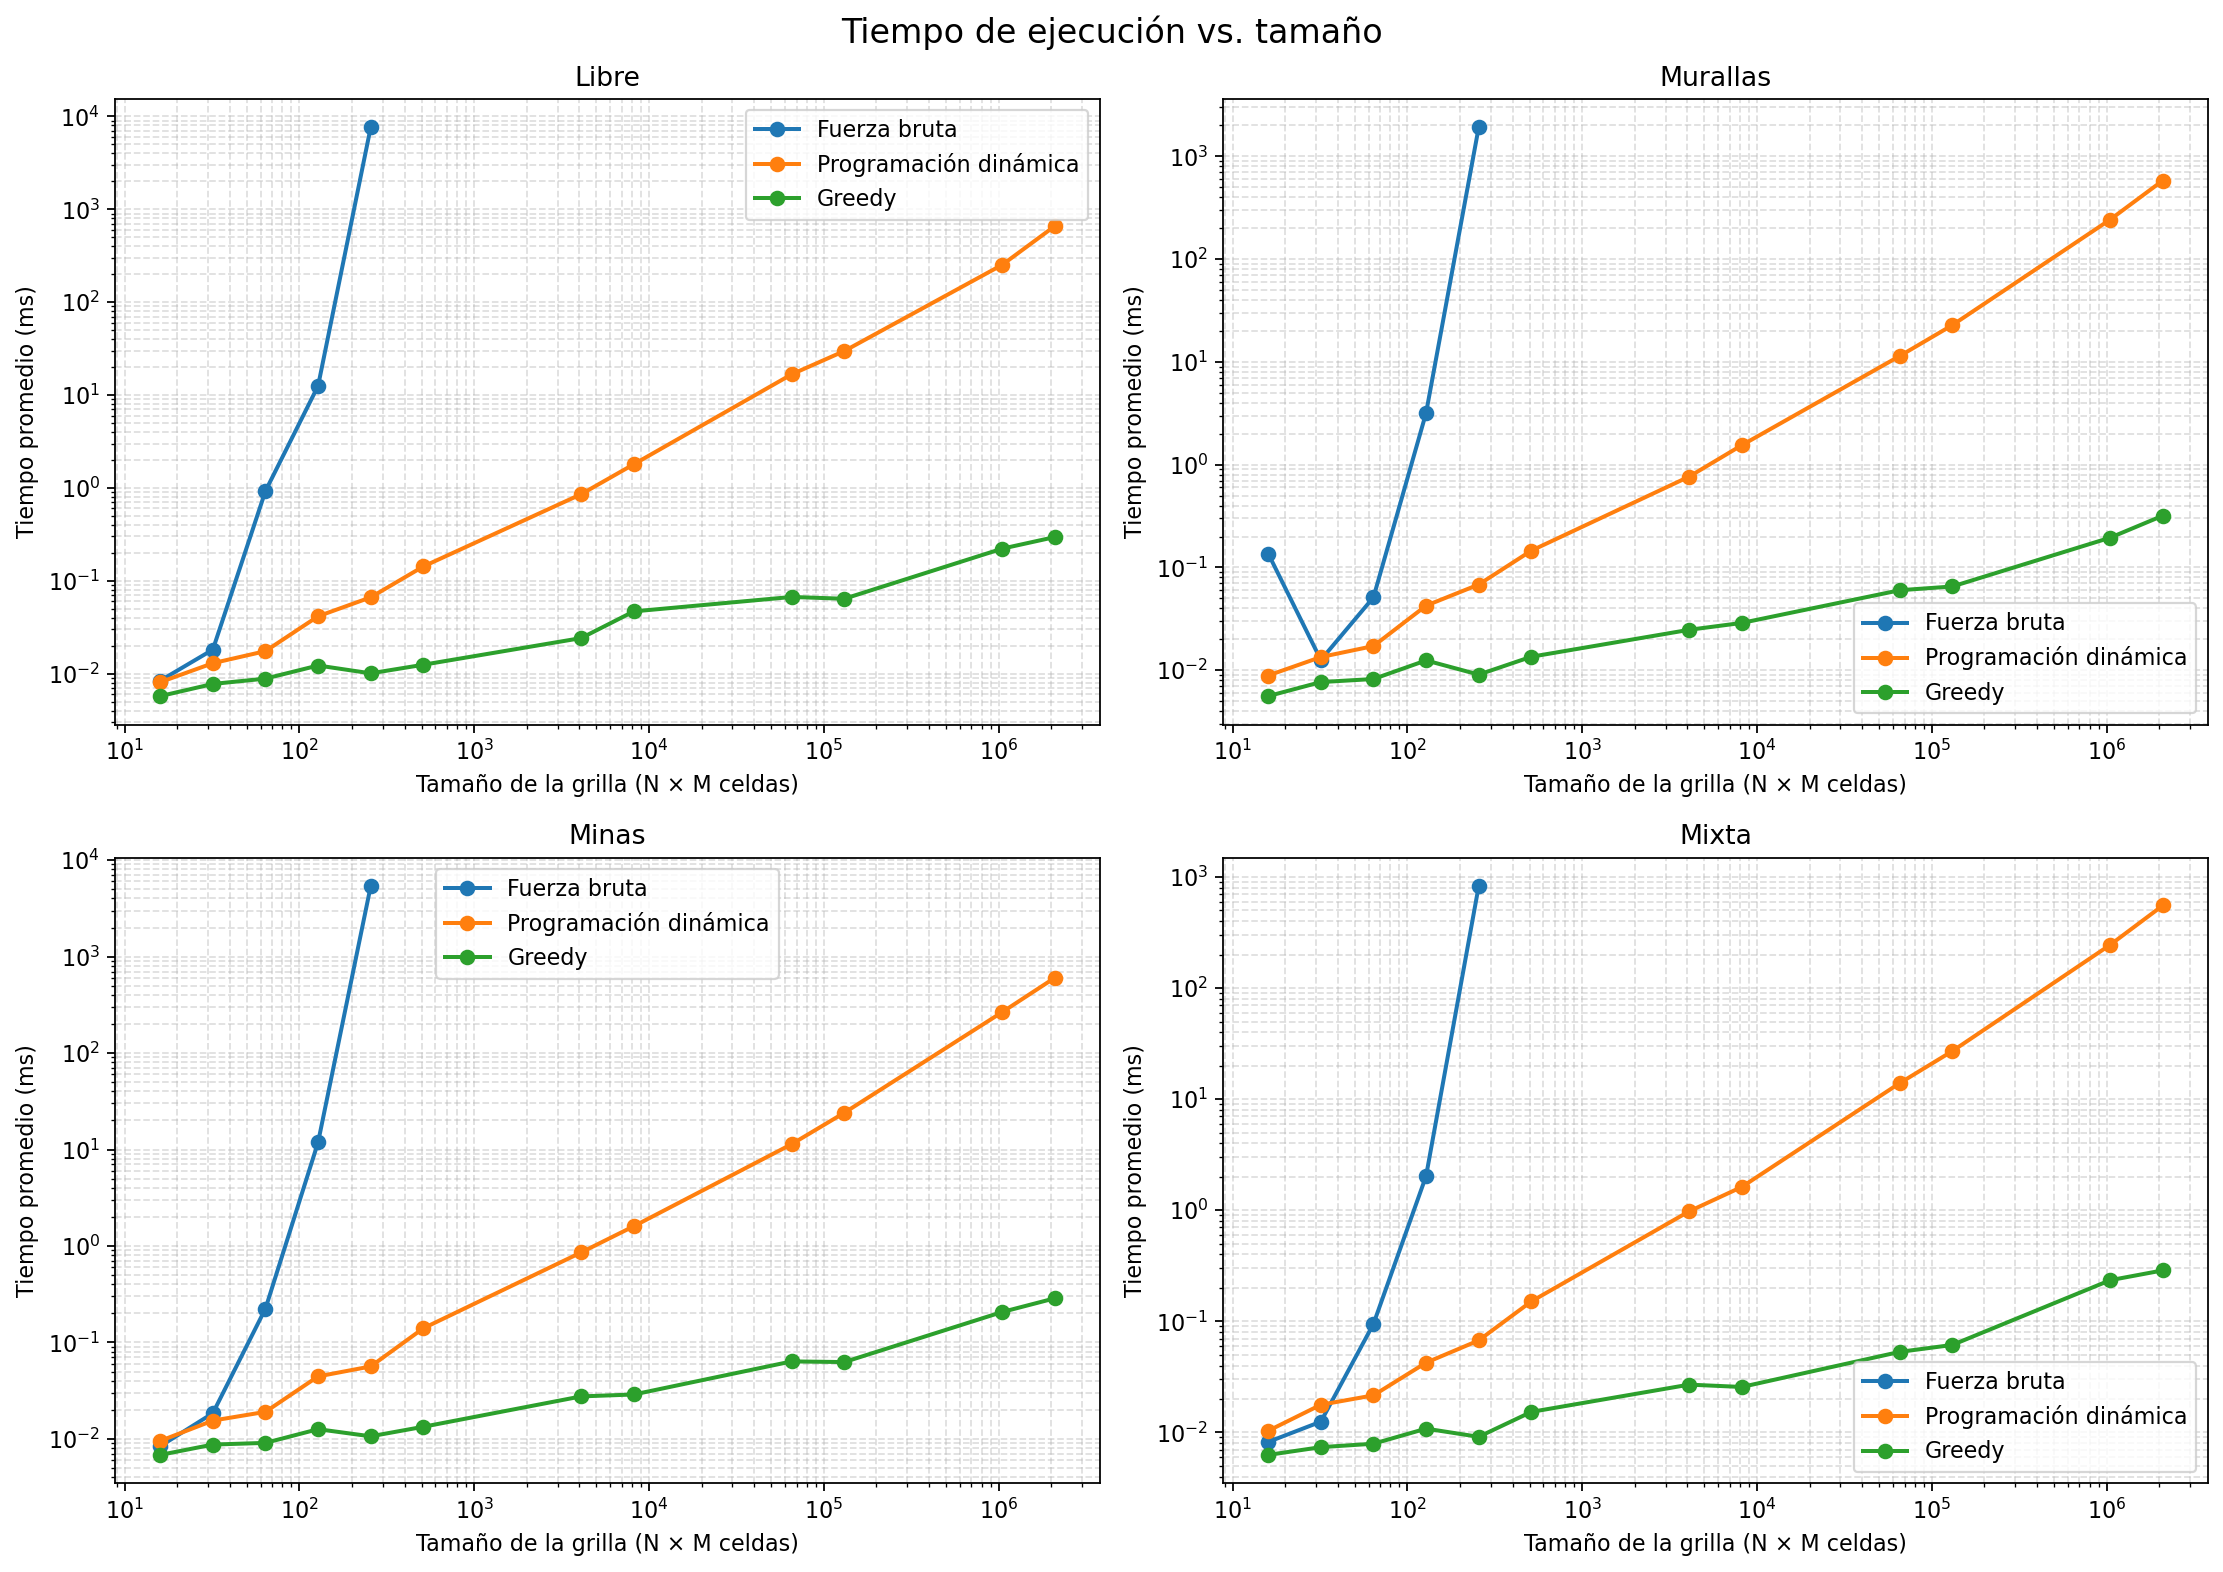
\includegraphics[width=0.85\textwidth]{../code/grid_pathfinding/data/plots/tiempo_ejecucion.png}
    \caption{Tiempo de ejecución de los algoritmos vs. dimensión $n \times m$.}
    \label{fig:tiempo_ejecucion}
\end{figure}

\newpage

\subsection{Uso de memoria}

En la Figura~\ref{fig:uso_memoria} solo DP es visible: su 
memoria crece linealmente con el número de celdas hasta 
$\approx 2{,}3 \cdot 10^{5}$ KB, coherente con 
$\mathcal{O}(n \cdot m \cdot v)$. Esto equivale a 
aproximadamente $110$ bytes por celda, más que los datos puros, 
porque las tablas se almacenan como vectores 
anidados con muchas asignaciones pequeñas. 

\vspace{0.4cm}

Fuerza bruta y greedy usan $\mathcal{O}(n+m)$ 
(pila de recursión y camino) y quedan en aproximadamente $0$ KB, 
que estan representados en los graficos como una recta horizontal
en el valor de $0$ KB para los 4 graficos.

\begin{figure}[H]
    \centering
    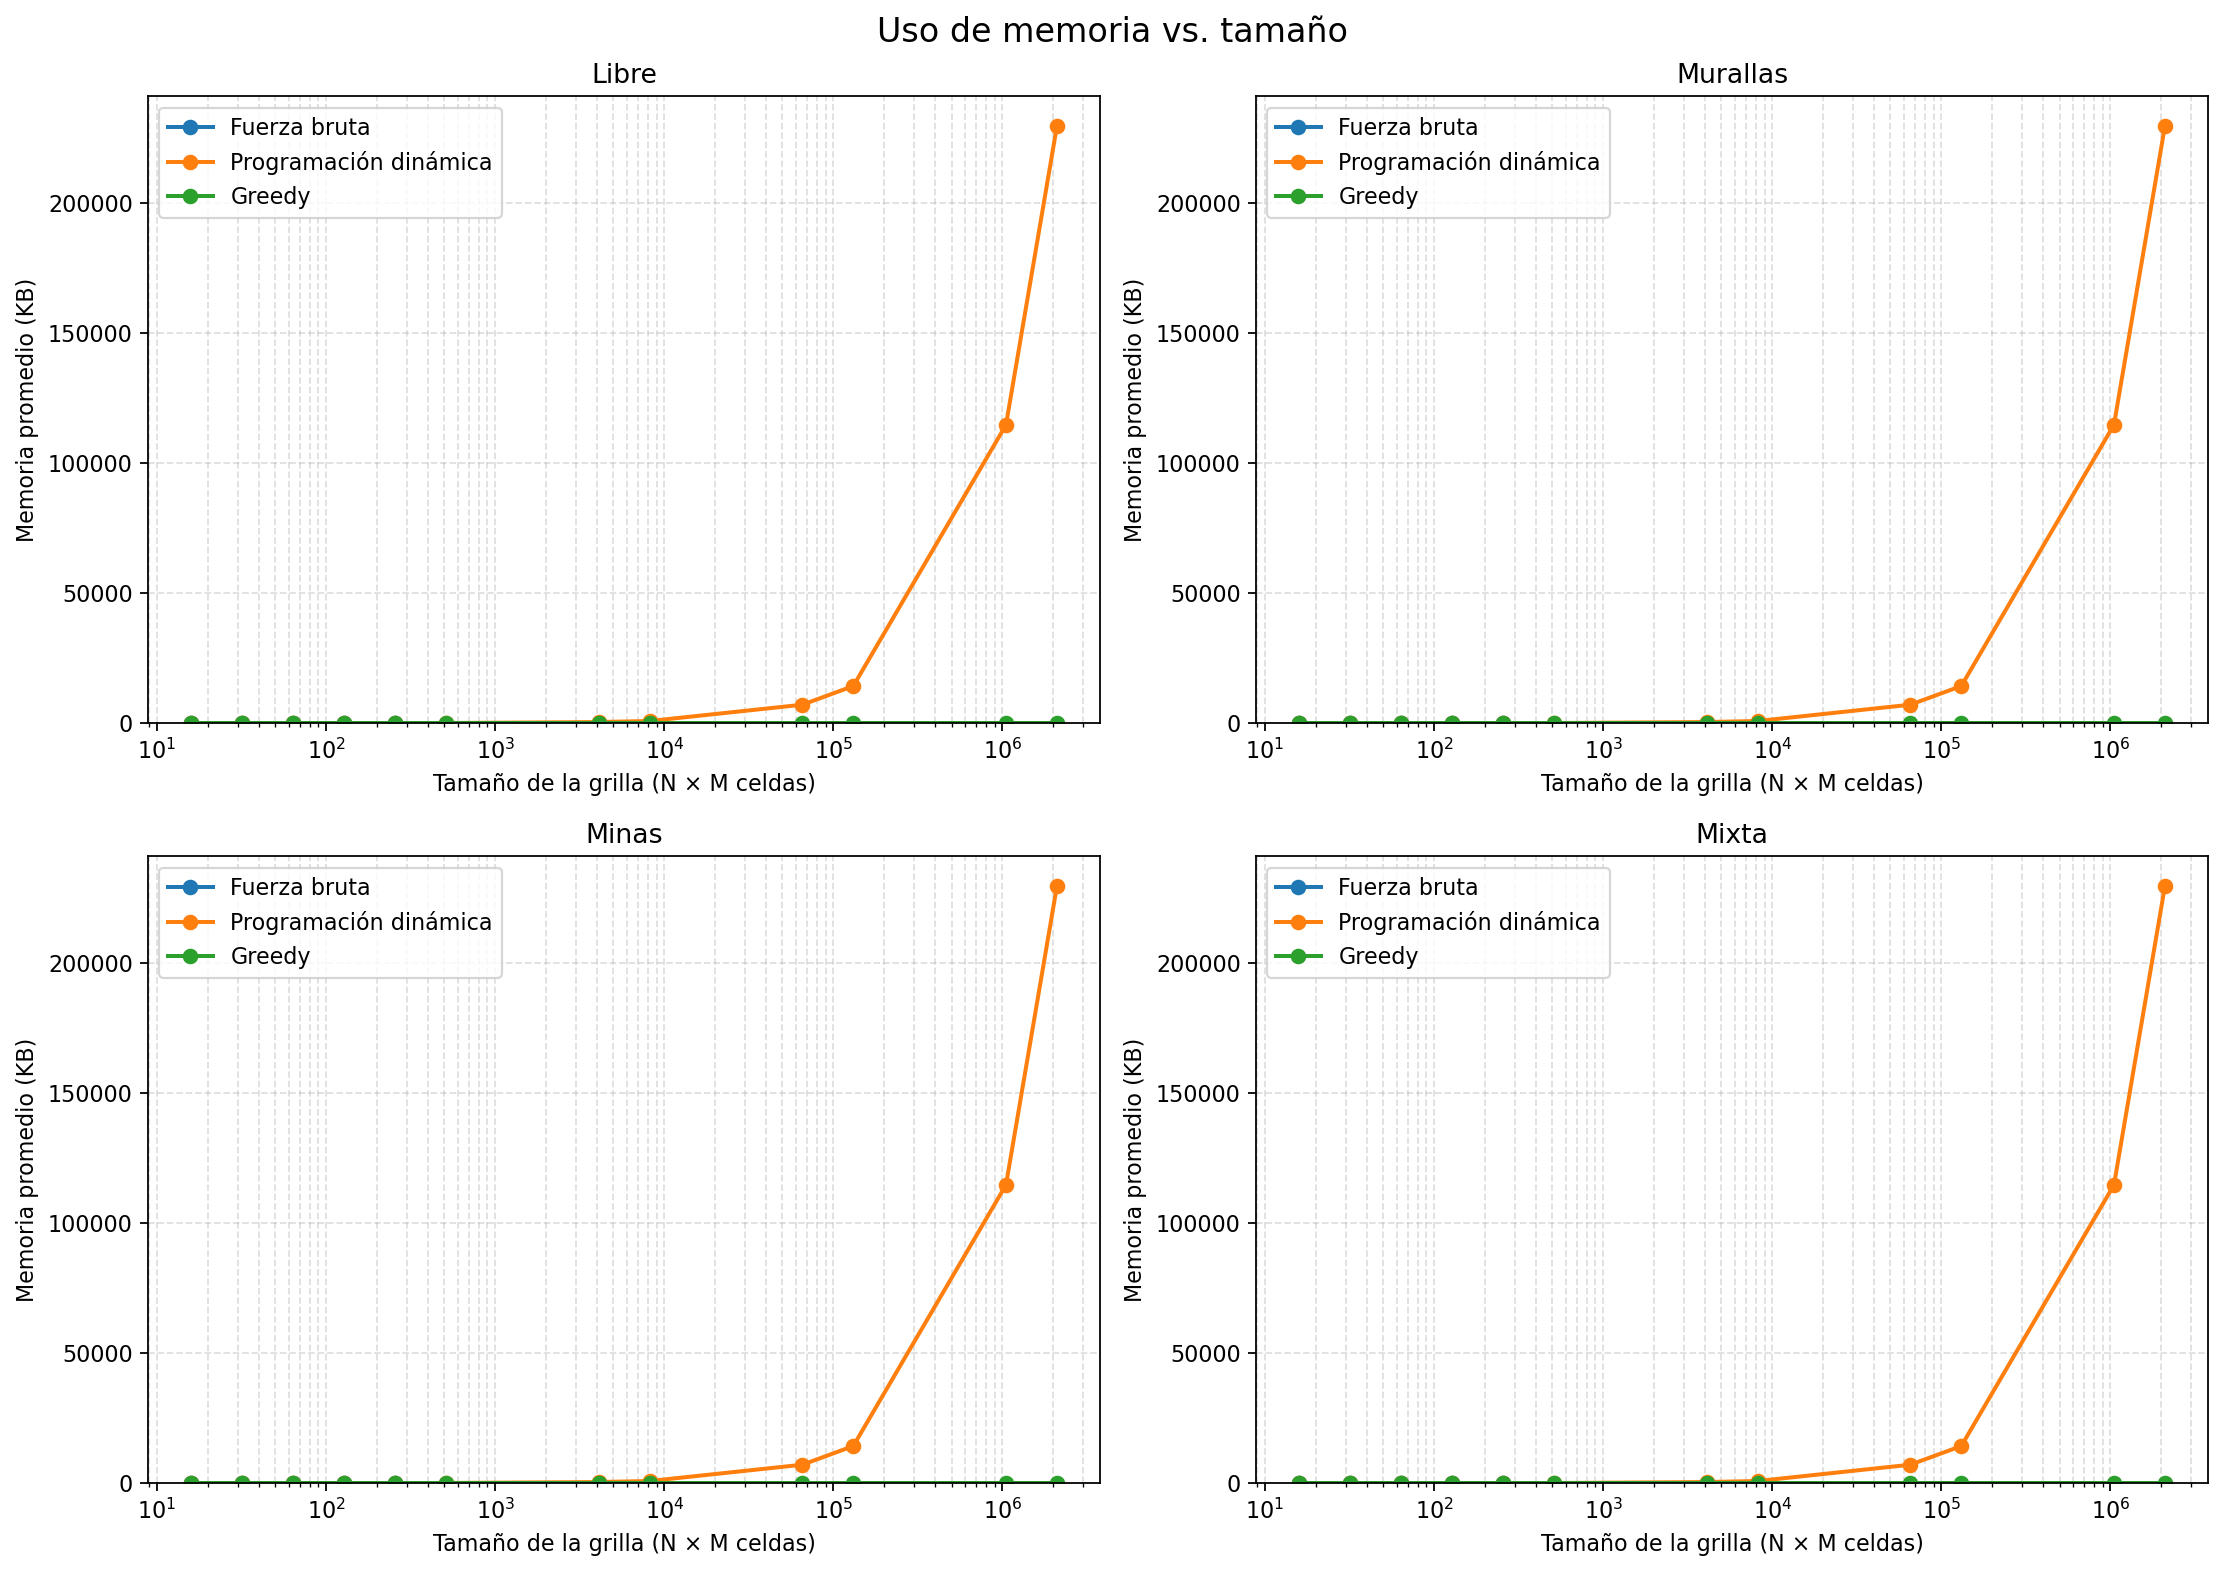
\includegraphics[width=0.85\textwidth]{../code/grid_pathfinding/data/plots/uso_memoria.png}
    \caption{Uso de memoria de los algoritmos vs. dimensión $n \times m$.}
    \label{fig:uso_memoria}
\end{figure}

\newpage

\subsection{Calidad de las soluciones de greedy}

La Figura~\ref{fig:brecha_greedy} muestra la brecha 
$\Delta = s(C^*) - s(C_{\text{greedy}})$, calculada 
cada vez que greedy consigue llegar a la meta y tomando 
como óptimo el puntaje de DP (eje vertical en escala symlog). 
$\Delta$ crece con el tamaño en los cuatro terrenos: de 
aproximadamente $10^{0}$--$10^{1}$ en las grillas más pequeñas a 
aproximadamente $10^{4}$ (D10) y $10^{5}$ (D1000) en $1024 
\times 2048$. La pendiente en escala log-log es cercana 
a $1/2$ respecto del número de celdas, es decir, $\Delta$ 
crece aproximadamente de forma lineal y proporcional a $n+m$: greedy pierde 
una cantidad parecida por paso y esa pérdida se acumula.

\vspace{0.4cm}

La curva de D1000 queda unos dos órdenes de magnitud 
sobre la de D10, coherente con que los valores y la 
penalización escalan $\times 100$. Las irregularidades 
de Murallas D1000 en grillas pequeñas se deben a que cada 
punto promedia a lo sumo 3 instancias y, en esas 
dimensiones, greedy además puede no encontrar un camino valido en gran parte de ellas, por lo que 
$\Delta$ se calcula con pocos casos.

\begin{figure}[H]
    \centering
    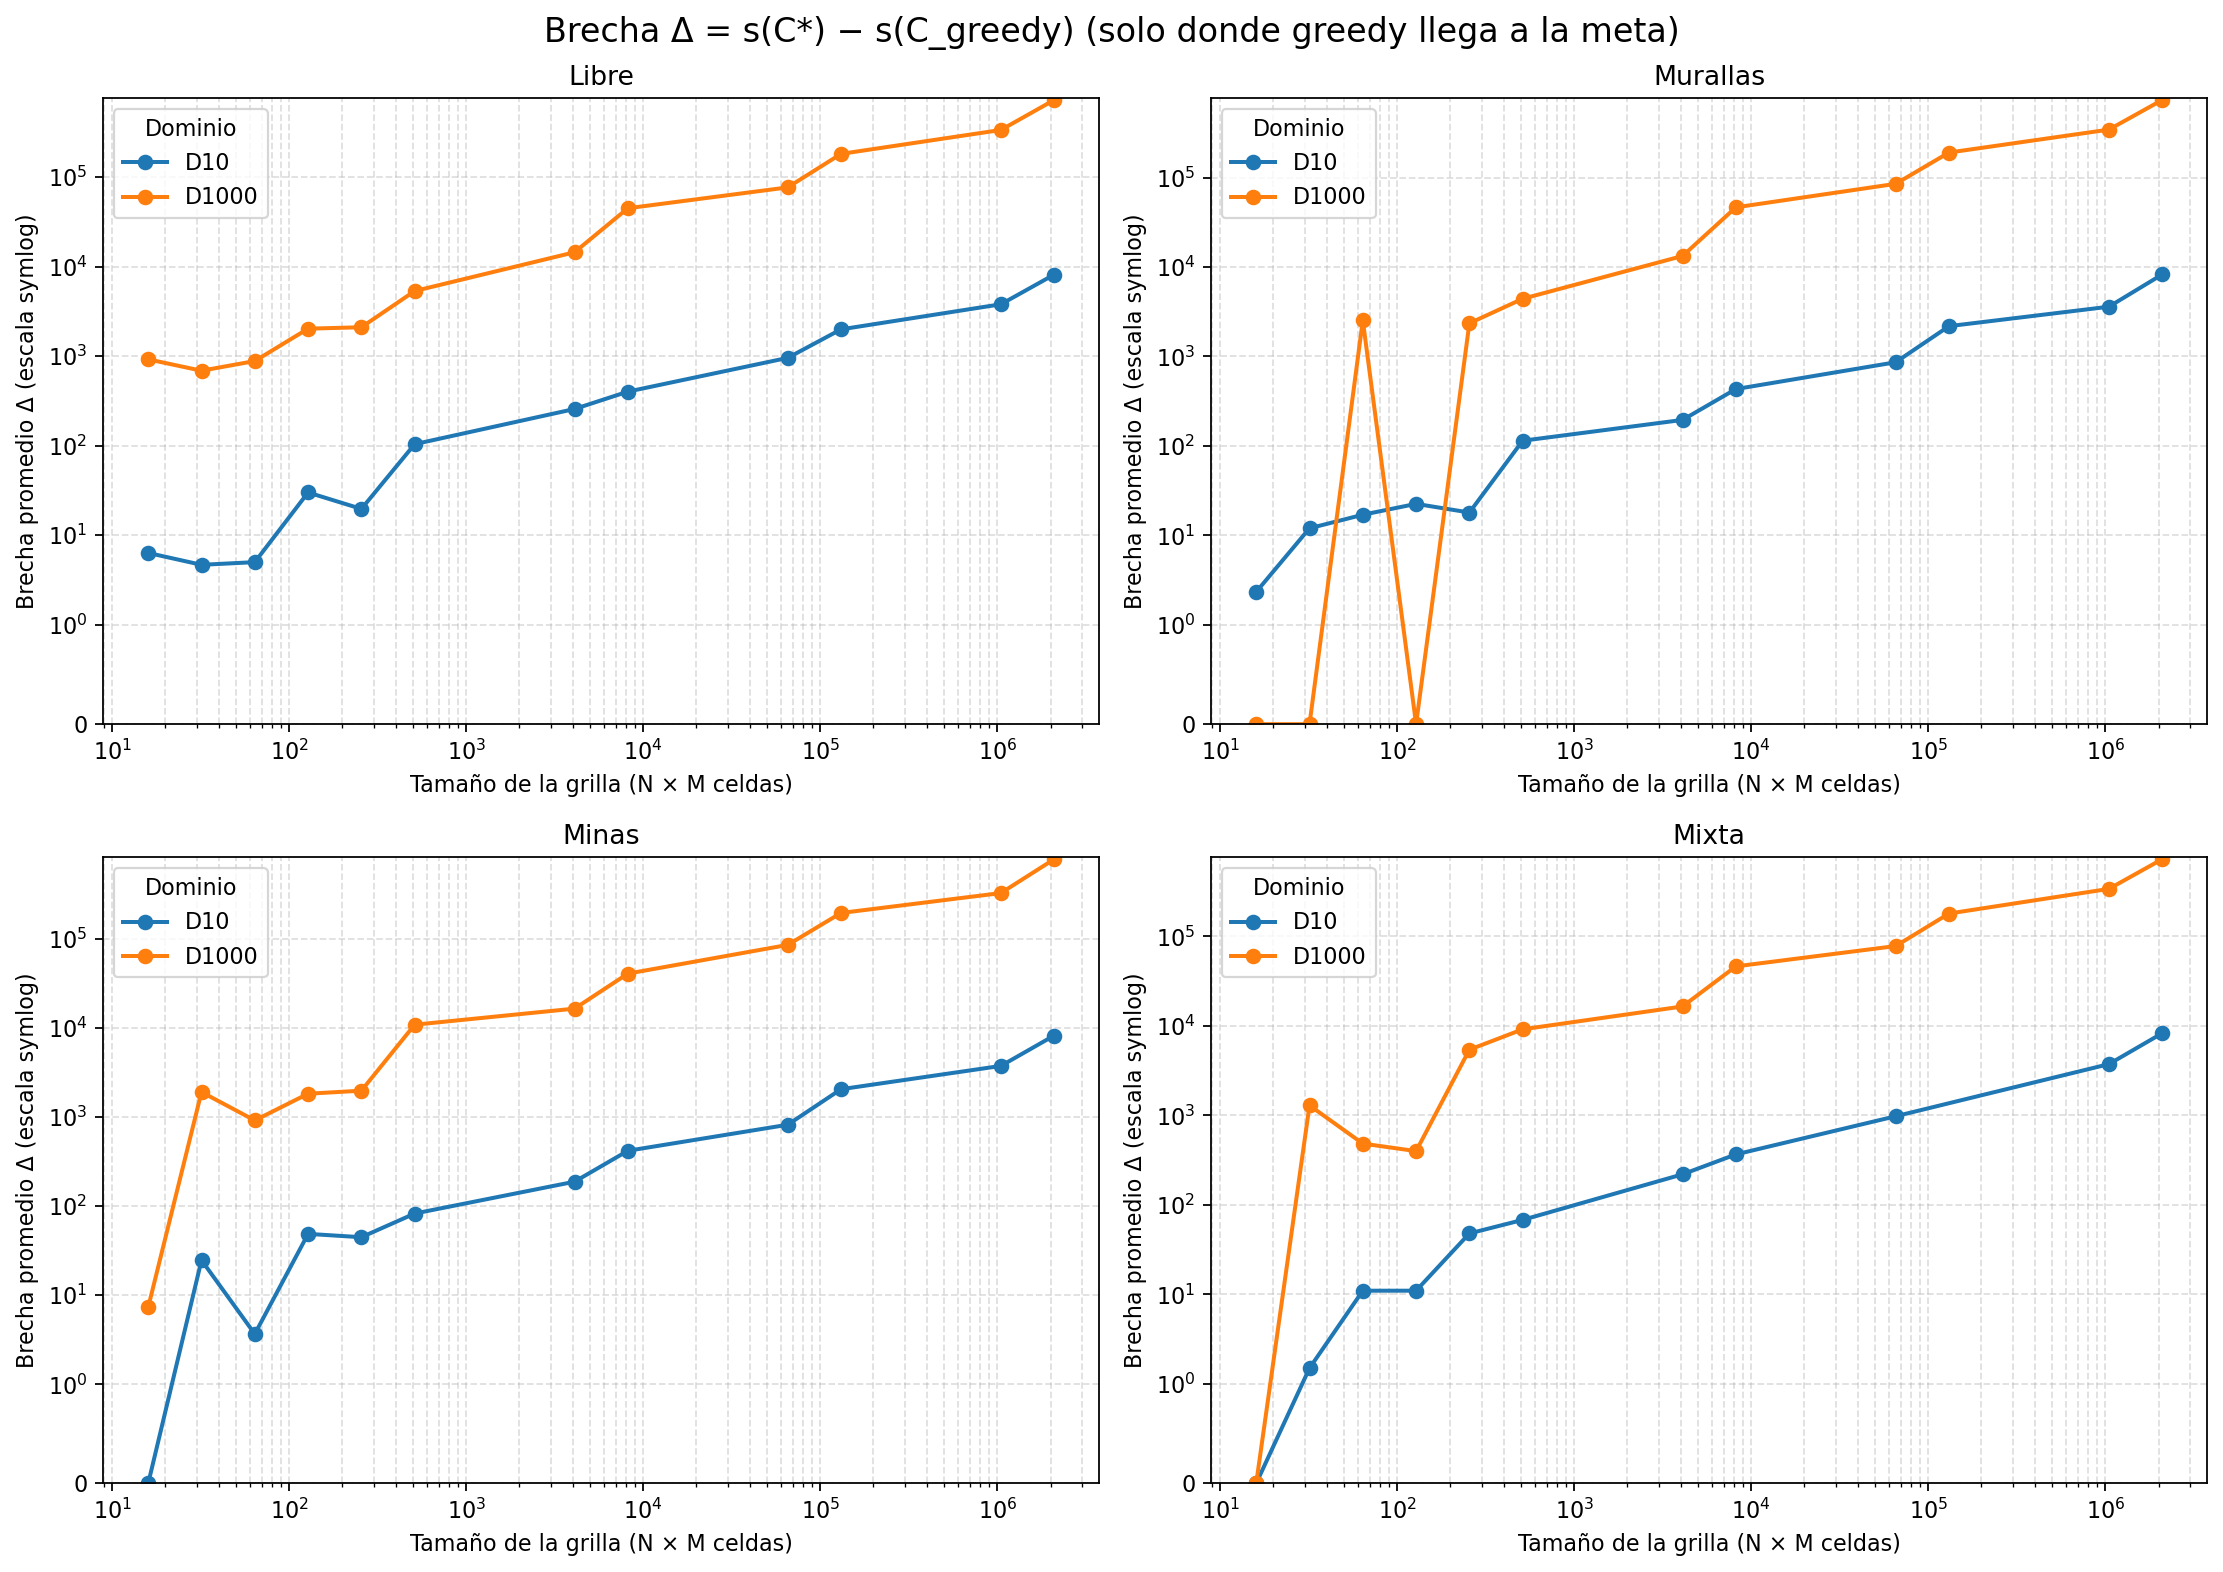
\includegraphics[width=0.85\textwidth]{../code/grid_pathfinding/data/plots/brecha_greedy.png}
    \caption{Brecha del algoritmo greedy vs. dimensión $n \times m$.}
    \label{fig:brecha_greedy}
\end{figure}

La Figura~\ref{fig:tasa_falla_greedy} muestra la tasa de 
falla, definida sobre las instancias que tienen solución 
según DP. En terreno libre es $0\%$ en todos los tamaños, 
lo que tiene sentido porque sin muros ni minas greedy siempre tiene 
un movimiento válido. En minas es prácticamente $0\%$ 
(un único punto de $33\%$ para D10). En murallas y 
mixta la falla es frecuente (varia de $33$--$67\%$, y $100\%$ 
en un punto de mixta D10), sin tendencia clara con el 
tamaño. 

\vspace{0.4cm}

Como cada punto agrupa 3 semillas, la tasa solo 
toma los valores $0\%$, $33\%$, $67\%$ y $100\%$; las 
oscilaciones reflejan variabilidad entre instancias y 
no un efecto del tamaño. La causa es que greedy mira un 
solo paso adelante y puede entrar a un callejón sin 
salida junto a los muros. Con minas casi no falla, 
tiene sentido porque la penalización $p$ hace poco 
factible pisarlas cuando hay alternativa, y por esto
rara vez agota las 3 vidas.

\begin{figure}[H]
    \centering
    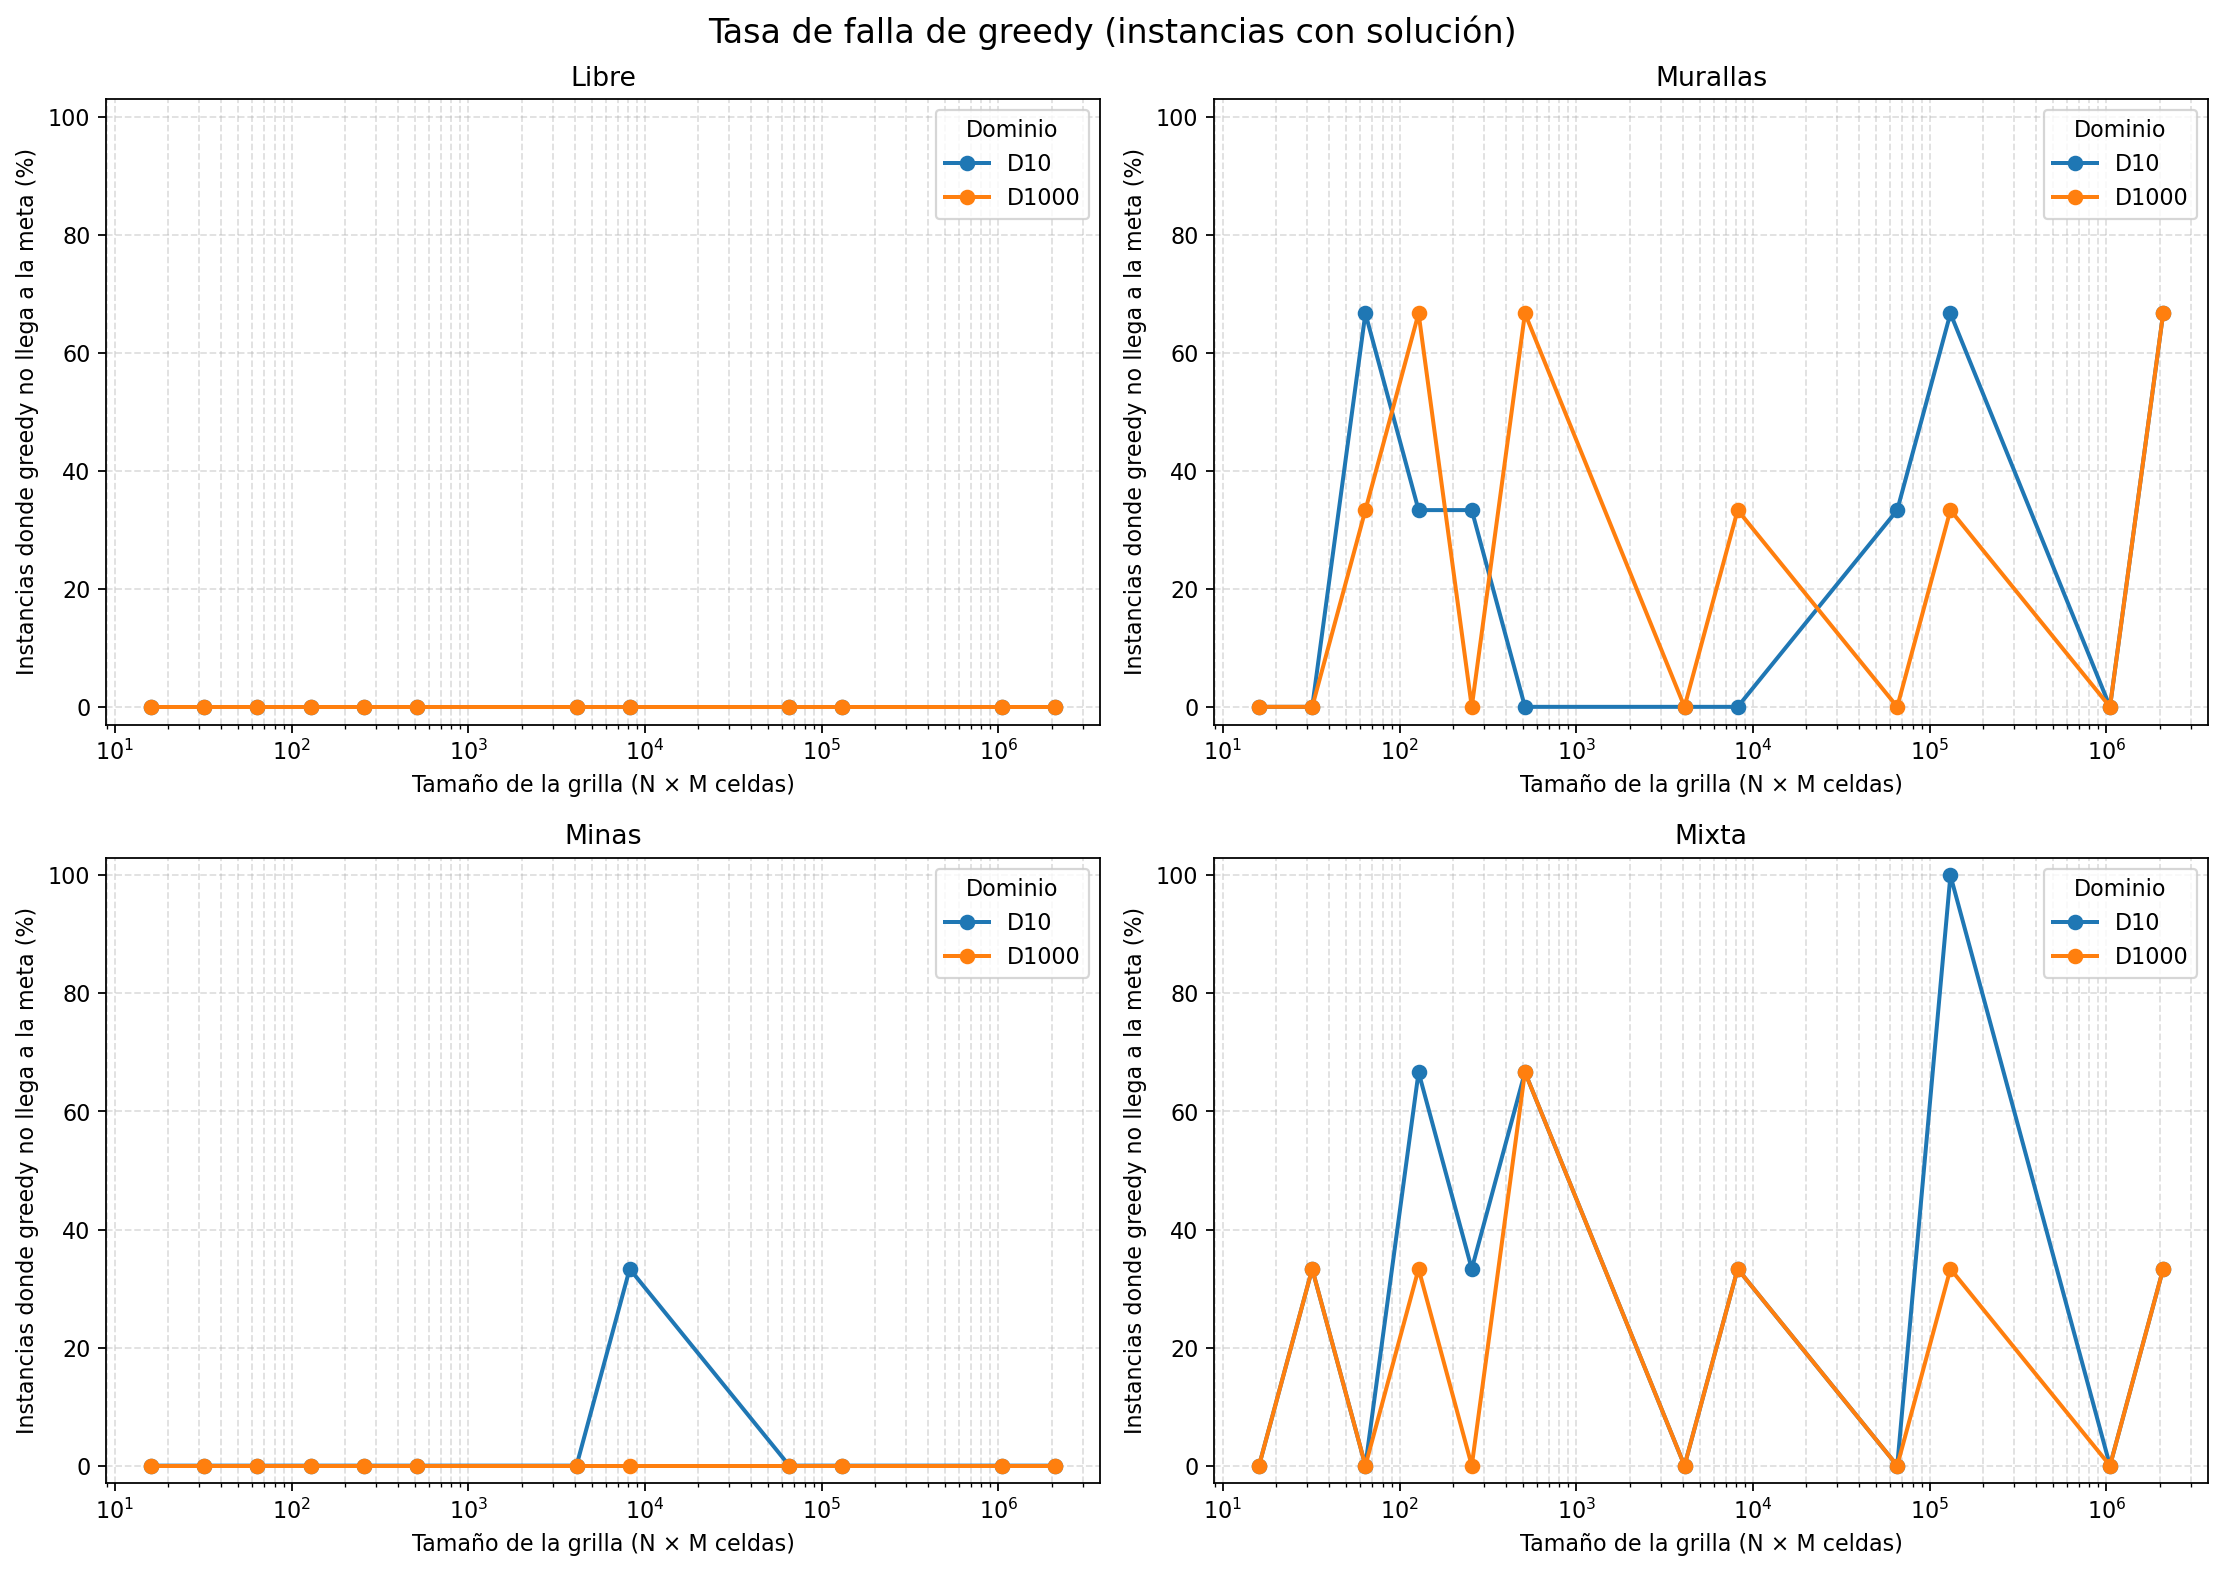
\includegraphics[width=0.85\textwidth]{../code/grid_pathfinding/data/plots/tasa_falla_greedy.png}
    \caption{Tasa de falla del algoritmo greedy vs. dimensión $n \times m$.}
    \label{fig:tasa_falla_greedy}
\end{figure}